

\documentclass[conference]{IEEEtran}

\usepackage{graphicx,color}
\ifCLASSINFOpdf
  % \usepackage[pdftex]{graphicx}
  % declare the path(s) where your graphic files are
  % \graphicspath{{../pdf/}{../jpeg/}}
  % and their extensions so you won't have to specify these with
  % every instance of \includegraphics
  % \DeclareGraphicsExtensions{.pdf,.jpeg,.png}
\else
  % or other class option (dvipsone, dvipdf, if not using dvips). graphicx
  % will default to the driver specified in the system graphics.cfg if no
  % driver is specified.
  % \usepackage[dvips]{graphicx}
  % declare the path(s) where your graphic files are
  % \graphicspath{{../eps/}}
  % and their extensions so you won't have to specify these with
  % every instance of \includegraphics
  % \DeclareGraphicsExtensions{.eps}
\fi



% correct bad hyphenation here
\hyphenation{op-tical net-works semi-conduc-tor}


\begin{document}

\title{Planning Paths for Rats using Actor-Critic Model}


\author{Zachary DeStefano}

% make the title area
\maketitle


\begin{abstract}
For this project, I attempted to see what paths a rat would take if the Morris Water Maze contained multiple rewards of varying value. The inspiration for this project was the layout of cities and the transportation networks used to connect them. I hoped to observe if a trained rat would use paths that look similar to those transportation networks. In order to do this, I trained the rat using hippocampal place cells that learn via temporal difference learning in the actor-critic model. After training, I started the rat at random locations and recorded the paths it took to the reward centers. In the end, the paths are suboptimal thus rats should not be used for path planning. 
\end{abstract}

\IEEEpeerreviewmaketitle



\section{Introduction}

The Morris Water Maze is one where a rat is released into a pool of water and searches for a platform which will provide relief from having to swim. The platform is thus considered a reward in the brain of the rat. Due to the constant location of these platforms, it is optimal for the rat to learn this location. By observing the rat over multiple trials we can extrapolate information about its learning abilities.\\
\\
If we wish to approximate what would happen if we did a physical experiment, we can use a model for its neuronal activity. For the purposes of this experiment, I assumed that there are a series of place cells in its hippocampus that each have their own actor and critic cells. The place cells fire at their own preferred locations and send signals to the actor and critic cells. When the rewards are reached, the actor and critic values are updated using the Temporal Difference learning rule. Output from the actor and critic cells is used to determined the rat's next move. The neuronal network described was implemented by Foster et al \cite{foster}. \\
\\
In the paper by Foster, they had a single reward center for the rat. For this experiment, I wanted to observe what could happen if you used the same neuron model but had multiple reward centers. More specifically, I wanted to observe the paths that a rat would take to travel between all the reward centers. The hope is that something similar to a Steiner Tree \cite{steiner1,steiner2} would emerge. 

\section{Related Work}

\subsection{Steiner Tree Problem}

The Euclidean Steiner Tree Problem is as follows: Given $n$ points in a $2D$ plane, connect them via line segments such that the total line segment length is minimized and every point can travel to every other point. Currently this problem is NP-hard meaning that it is not known whether or not there is an efficient algorithm. There is a polynomial time approximation scheme that has been found for it \cite{steiner1,steiner2}.  

\subsection{Slime Mode Interstates}

There was an attempt at solving something similar to the Steiner Tree problem using the behavior of biological organisms. Food was placed at locations imitating the 20 largest cities in the United States and then slime mold was released \cite{slimemold}. The paths sketched out by the slime mold ended up being similar to the interstate highway system and is thus likely similar to what the Steiner Tree would look like. This is a great example of how the aggregate of simple actions taken by a biological organism can yield useful results. My goal with the rat experiment was to see if we would get useful results taking the aggregate of the paths it takes after learning. 

\subsection{DA-STDP for foraging tasks}

Another model that has been proposed in the literature to simulate reinforcement learning is Dopamine-modulated Spike-time dependent plasticity (DA-STDP). There are two papers in particular where they used it to model a direct actor foraging for rewards. \\
\\
In a paper by Skorkheim et al \cite{plosone}, they model an actor foraging for food using DA-STDP. As it turns out, DA-STDP can be used to model the behavior effectively, however you have to impose additional constraints related to maintaining synaptic homeostasis in order for it to be effective. A similar experiment was done by Evans \cite{robot}, where he modeled the movement of a robot foraging for food in an environment. \\
\\
These papers indicate that it may be possible to use DA-STDP to model the rat's behavior in my environment. However, there are two key differences between my set-up and those papers. First, in my experiment, the input is place cells thus the rat knows its global location. In those papers, the input is the immediate environment around the actor at a given point. The second major difference is that both experiments have many food items spread around the environment and it does not matter which food items the actor receives. For my experiment, I only had a few reward centers and I was aiming for the actor to visit all of them. \\
\\
The lack of reward centers in my experiment would mean that the spiking would occur much less than in other papers that used DA-STDP. For this reason, training the rat to move around my maze would likely be impractical and infeasible. I thus decided to stick with the Actor-Critic Model for my purposes. 

\section{Experiment Design}

\subsection{Rat Movements}

For the real experiments there would be a rat moving around a circular pool. I thus had a "rat" with an x-y location moving around a circle. In my model, the rat has place cells in its hippo-campus and each of the place cells has a preferred location in the circle. Each place cell feeds into a critic cell as well as 8 actor cells. The place cell location, responses by the actor and critic cells, and final direction chosen by the rat was determined using the model specified in Foster et al \cite{foster}. \\
\\
There were two important things to consider when modeling the rat's movements: how much it changes direction and what to do if it hits the wall. For simplification, I assumed that a rat "bounces off" a wall if it hits it. This means that I had $\pi$ radians to its direction of movement in order to reverse it. When doing this, it is possible that if the rat hits the wall from a certain angle at the right location, then it could keep bouncing forever. If the rat failed to be at a proper location after "bouncing" then I change its direction by $\frac{\pi}{2}$ radians in order to prevent this from occurring. \\
\\
The other thing to consider is how much the rat's direction is allowed to change in each time step. Here I deviated from the design in Foster \cite{foster} and chose my own method. I assumed that in each time step, the rat has only three choices: continue traveling in the same direction, move slightly to the left, or move slightly to right. Traveling in the same direction means that the angle of movement stays constant. Moving slightly to the left means that the angle increases by $\frac{\pi}{4}$ radians. Moving slightly to the right means the angle decreases by $\frac{\pi}{4}$ radians. In order to determine the rat's next move, I shifted the coordinate system so that the previous angle was the positive x-direction. If the vector representing the next angle had a positive y-value then I had the rat move slightly to the left. If the vector had a negative y-value then the rat moved slightly to the right.\\
\\
**FIGURE OUT WHEN I DID NOT USE THIS**

\subsection{Rat Training and Rewards}

In order to train the rat, I followed the procedure used in Foster \cite{foster} and used many parts of the morris\_water\_maze.m code. In each trial, the rat was released in one of 4 locations and then "moved" (as described above) until it found a reward center or 250 time steps had passed, whichever came first. Once the reward center was found, the actor critic values were updated. Unlike in Foster \cite{foster}, I had multiple reward centers. Initially they all gave a reward of 1.\\
\\
In order to make sure a rat does not get too attached to one reward, their reward value decreased by a constant amount each time the rat reached it. The reward center was not used once the value fell below a certain threshold. The rat was trained until a certain number of trials occurred or all the rewards had been spent, whichever came first. \\
\\
In order to see if there would be an effect if we modeled the fact that cities have different populations, I also ran trials where the initial reward values were different. I took the population values and did a rescale and shift so that they fell between 0.5 and 1. 

\subsection{Reward Center Locations}
For the reward center locations, I used basic locations to start off and then used locations inspired by the cities in the United States and Europe. \\
\\
In order to have well placed cities, for my United States map, I used New York, Chicago, Los Angeles, Atlanta, and Denver. For the Europe map, I used Warsaw, Berlin, and Vienna. I found their latitude and longitude coordinates in signed degrees format and plotted them on a 2D plane, rescaling for the water maze. I made sure to vary which particular set of cities I chose in a given trial. 

\subsection{Rat Testing}

Once the rat was trained, I recorded the paths it takes when released back into the maze. The rat movement was exactly the same as during training except that the actor and critic values were left unchanged. The rat also started at random locations in the maze. In order to model a random location, I used polar coordinates and chose random $\theta$ and $r$ values that are within the realm of the circle and then converted the $(r,\theta)$ pair to its corresponding $(x,y)$ pair. During testing, I just wanted to see all the different paths a rat would take thus it did not stop at a reward center and just kept moving in the direction the actor told it to move.

\section{Results}

\subsection{Intiial Runs}

For this experiment, it was critical to learn the actor gradients at each of the place cell. This would give a good indication as to the preferred direction of the rat at each point and thus indiciate which direction it is most likely to travel. When there was only one reward as in Foster et al \cite{foster} **VERIFY THIS CLAIM**, the gradients tended to point toward the reward after learning. For my experiment, I was hoping they would all point to the nearest reward out of multiple rewards. Unfortunately, this did not always happen. \\
\\
When I first ran the experiment, I did not do any foraging behavior and thus kept the reward values constant. This would often cause the rat to favor the first reward it found and there would be an imbalance in that the actor gradients all favored that reward. Even when it did reach other rewards, the weights from the initial reward were great enough that the model still favored it. \\
\\
Another issue that emerged occured when the rat reached different reward centers a roughly equal amount of times and there was a distinct region between the reward centers where the gradient direction does not favor one reward center too strongly. When I ran the simulation after this occurred, instead of the rat randomly choosing one of the regions as I had hoped, it would instead become stuck between regions and move in a zig-zag manner near the border. This issue was not entirely mitigated and in my results are cases where the zig-zag motion can be observed.\\
\\
After using depreciating rewards, the rat starting moving around the maze in a more logical manner yet still with wide variations. The actor gradients still tended to favor one of the reward centers but not as highly as had happened before. The issue with the rat being unable to choose at border areas still persisted. When the paths were mapped, there were mixed results. In some cases, the highest density of path lines occurs in the path between reward centers which is exactly what we want. In other cases, the density of path lines is vaguely close to that but the movement of the rat was much more erratic than desired.

\subsection{European cities, constant initial rewards}

For the first figure, figure 1, the reward center locations reflect the European cities mentioned in the Reward Center Locations subsection of my experimental design. For this run, I depreciated the rewards by a constant factor in each time step. The reward values were all uniform in the beginning. After training, the actor gradients tend to favor the rightmost reward center but still point to the other reward center. When the testing was performed the rat moved toward each of the cities but mostly stayed in the path between the cities. An interesting result was that the area between the cities had the more dense concentration of path lines, however one reward center had a much more dense concentration than the others. For the critic weights, as can be observed in figure 1, they were higher near the reward centers as expected, but areas nearest the rightmost reward had much higher critic values.

\begin{figure}
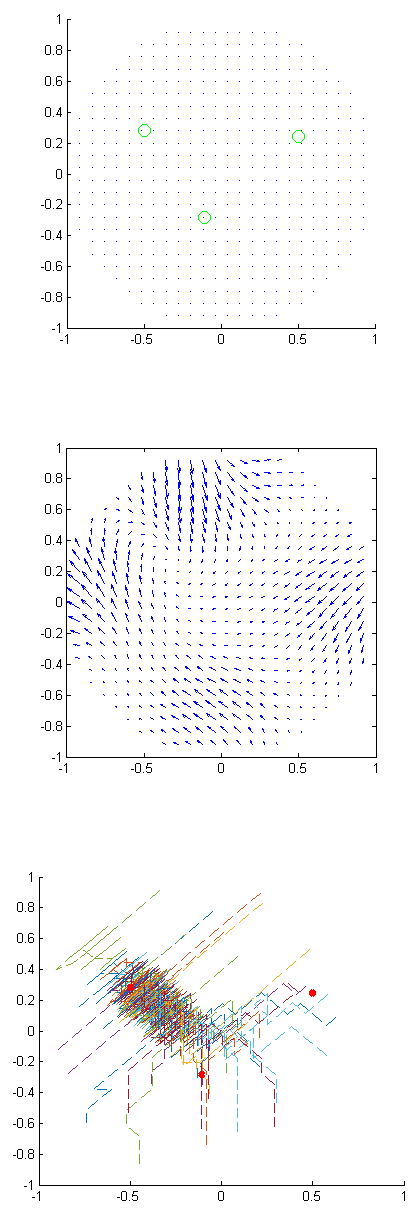
\includegraphics[width=0.4\textwidth]{waterMazeRevised2_Figure.png} 
\caption{Place Cells as blue dots and Reward Center Locations as green circles (top). Actor Gradient for each place in maze (middle). Paths traversed by rat with reward centers in red (bottom)}
\end{figure}

\begin{figure}
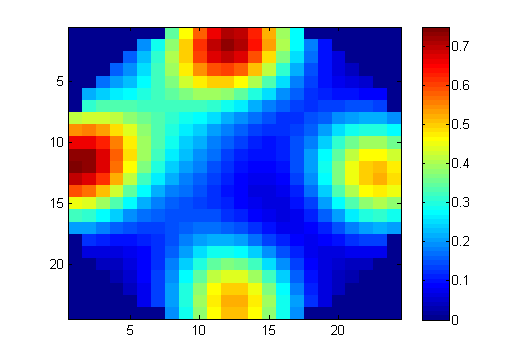
\includegraphics[width=0.4\textwidth]{waterMazeRevised2_Critic.png} 
\caption{Critic Weights for Maze from Figure 1}
\end{figure}

\subsection{American cities, constant initial rewards}

For Figure 3, the reward center locations reflect the American cities mentioned in the experimental design. The initial rewards are constant but they decrement by a constant amount instead of constant factor each time the rat receives it. The results ended up quite similar to the case of European cities. There ended up being a distinct area between the reward centers heavily favored by the actor gradient so during testing that area is densest in terms of path lines. Instead of heavily favoring one reward center over another, the rat seemed confused in this area. In Figure 4, the critic values are highest on the right or left side and low in the middle which probably helps explain the fact that the rat had a hard time choosing there.

\begin{figure}
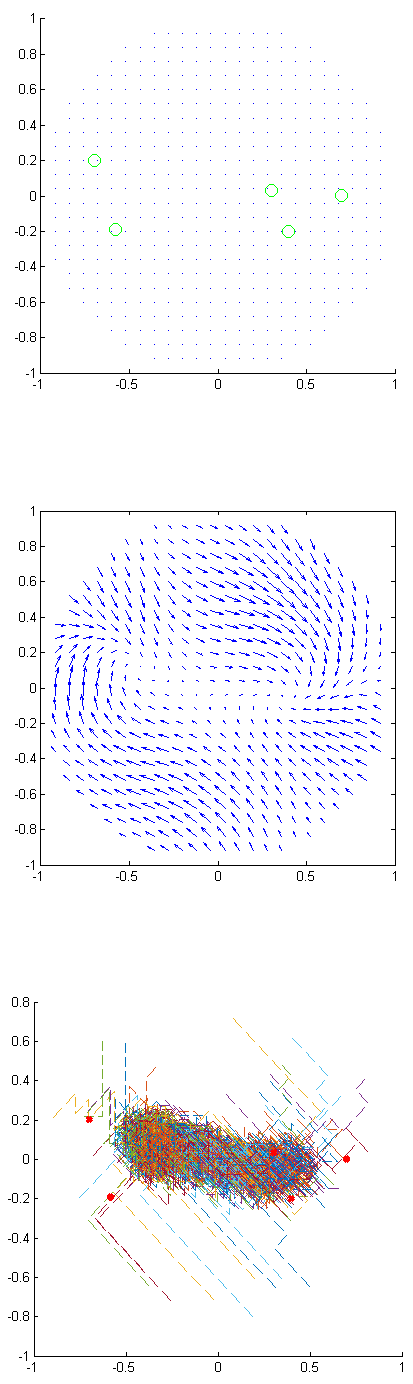
\includegraphics[width=0.4\textwidth]{waterMazeRevisedD_Figure.png} 
\caption{Place Cells as blue dots and Reward Center Locations as green circles (top). Actor Gradient for each place in maze (middle). Paths traversed by rat with reward centers in red (bottom)}
\end{figure}

\begin{figure}
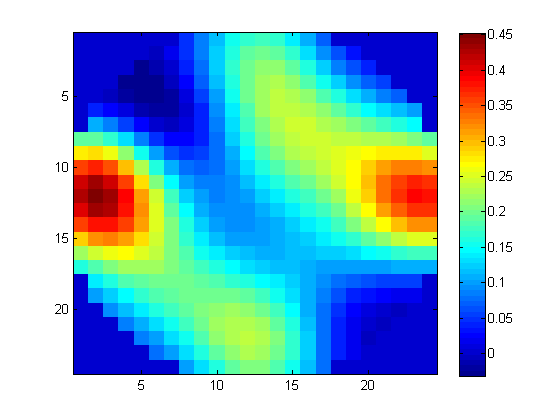
\includegraphics[width=0.4\textwidth]{waterMazeRevisedD_Critic.png} 
\caption{Critic Weights for Maze from Figure 3}
\end{figure}

\subsection{European cities, varying initial rewards}

For Figure 5, I used the European cities but changed their initial reward values based on their population. As can be observed, the results were not too different from before in that a strong preference exists for the area between the reward centers. The critic was similarly biased in Figure 6 toward one of the reward centers over the others.\\
\\
\begin{figure}
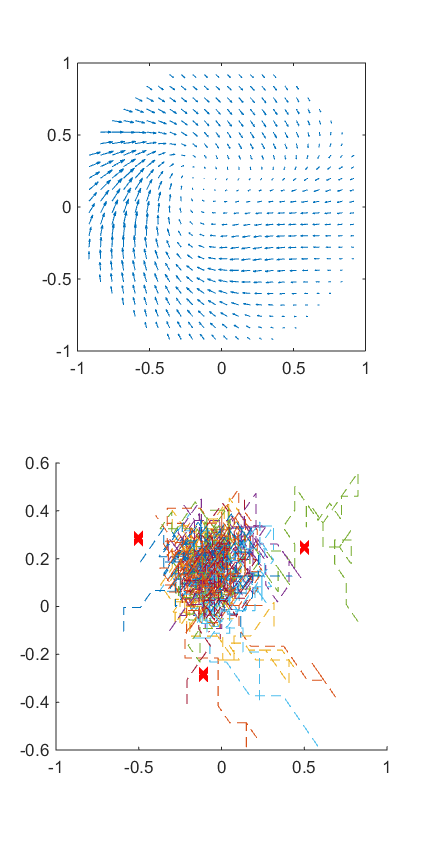
\includegraphics[width=0.4\textwidth]{waterMazeRevised2_Figure_populationRewards.png} 
\caption{Actor Gradient for each place in maze (top). Paths traversed by rat with reward centers in red (bottom)}
\end{figure}

\begin{figure}
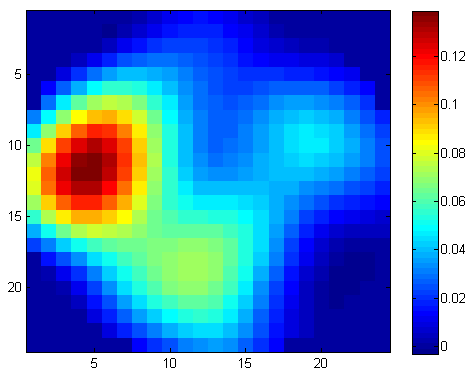
\includegraphics[width=0.4\textwidth]{waterMazeRevised2_Critic_populationRewards.png} 
\caption{Critic Weights for Maze from Figure 5}
\end{figure}

\subsection{American cities, varying initial rewards}

For Figure 7, I used the American cities but changed their initial reward values based on their population. Again, the results were not too different from before. There is a heavy amount of activity in the area between reward centers. In Figure 8, the critic heavily favored the right side over the left side of the maze.

\begin{figure}
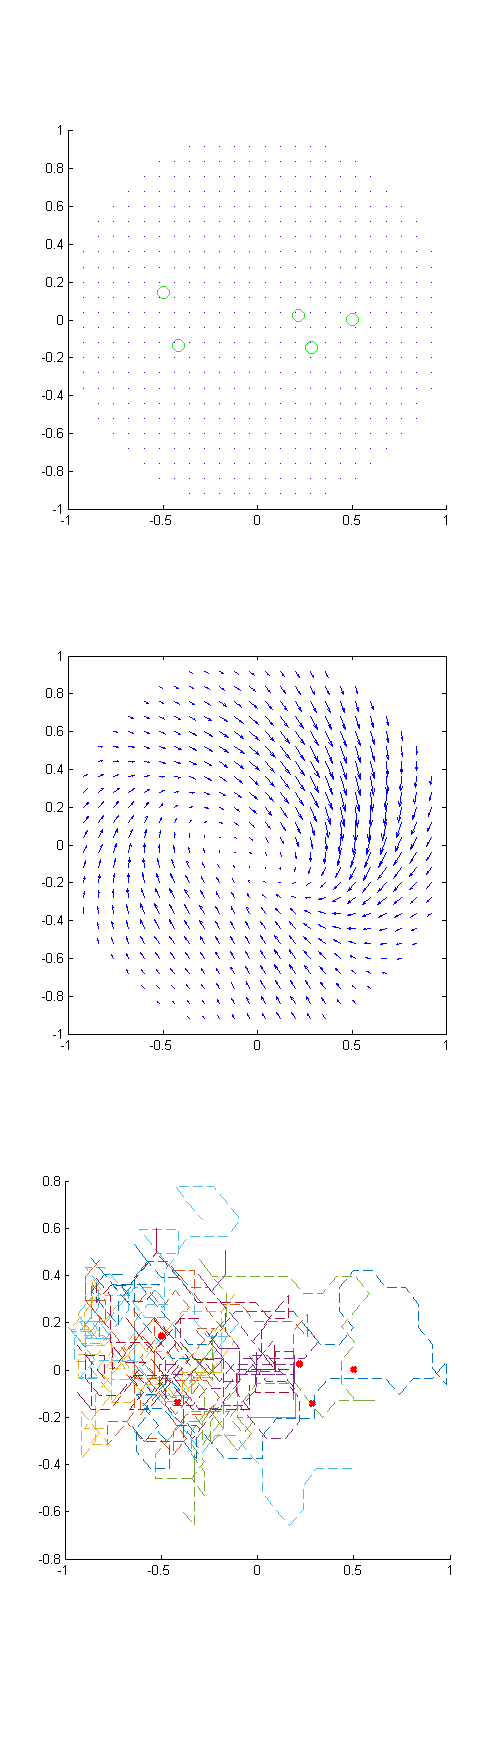
\includegraphics[width=0.4\textwidth]{waterMazeRevisedD_Figure_populationRewards.png} 
\caption{Actor Gradient for each place in maze (top). Paths traversed by rat with reward centers in red (bottom)}
\end{figure}

\begin{figure}
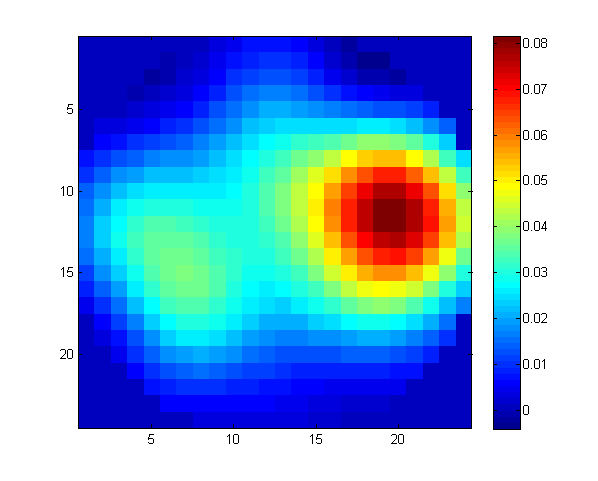
\includegraphics[width=0.4\textwidth]{waterMazeRevisedD_Critic_populationRewards.png} 
\caption{Critic Weights for Maze from Figure 7}
\end{figure}

\section{Conclusion and Future Work}

Rat should not be used for path planning or anything related to the Steiner Tree problem. The rat ended up with too much of a preference toward a particular reward center or it spent too much time in between reward centers unable to decided. Even after doing my best to overcome these adverse behaviors, the paths taken were not terribly informative. The best conclusion that could be drawn from the results is that the region with the densest concentration of path lines should contain a line segment in the Steiner Tree. Computing this line segment from the set of paths would be impractial though and the Steiner Tree approximation algorithm is definitely much more efficient than simulating the rat. \\
\\
My hope with this project was that the actor cells would point toward their nearest reward center if quite close to one and in other cases, compromise directions would be mapped out. After that if you released the rat in random locations and stopped the training, it would take a variety of paths to the various reward centers. The goal was that after mapping these paths, you would get a very dense concentration in a region that resembled a Steiner Tree. While there were concentrations in areas that are likely part of the Steiner Tree, I would be hestistant to conclude anything about what the Steiner Tree should look like from these rat paths. \\
\\
While there was no insight into the Steiner Tree problem through this project, I did gain insight into using the Actor-Critic Model with multiple rewards. The most ideal results occured with uniform starting values and decreasing rewards when the rat reached a reward center. The rat does learn paths toward reward centers but furthur effort is needed to ensure that a rat does not stay stuck between reward centers.\\
\\
The other possible extension of the multiple reward center work is using DA-STDP for the rat's behavior. The network would most reseble the one in \cite{plosone} however the input would be the place cell activity. The excitatory and inhibitory neurons as well as the output would likely stay the same for the most part with modifications to account for the number of place cell input neurons that I choose. As mentioned in the related work, the potential lack of spiking activity would however make this method potentially impractical.


%\bibliographystyle{acmsiggraph}
%\bibliography{finalPaperRefs}

\begin{thebibliography}{1}
\bibitem{slimemold}
Adamatzky, Andrew, and Andrew Ilachinski. "Slime mold imitates the United States interstate system." Complex Systems 21.1 (2012): 1.
\bibitem{steiner1}
Arora, Sanjeev. "Polynomial time approximation schemes for Euclidean TSP and other geometric problems." Foundations of Computer Science, 1996. Proceedings., 37th Annual Symposium on. IEEE, 1996.
\bibitem{steiner2}
Arora, S., "Nearly linear time approximation schemes for Euclidean TSP and other geometric problems," in Foundations of Computer Science, 1997. Proceedings., 38th Annual Symposium on , vol., no., pp.554-563, 20-22 Oct 1997
doi: 10.1109/SFCS.1997.646145
\bibitem{robot}
Evans, Richard. "Reinforcement Learning in a Neurally Controlled Robot Using Dopamine Modulated STDP." arXiv preprint arXiv:1502.06096 (2015).
\bibitem{foster}
Foster, D. J., R. G. M. Morris, and Peter Dayan. "A model of hippocampally dependent navigation, using the temporal difference learning rule." Hippocampus 10.1 (2000): 1-16.
\bibitem{plosone}
Skorheim S, Lonjers P, Bazhenov M (2014) A Spiking Network Model of Decision Making Employing Rewarded STDP. PLoS ONE 9(3): e90821. doi: 10.1371/journal.pone.0090821
\end{thebibliography}




% that's all folks
\end{document}


